% !TEX encoding = UTF-8 Unicode
\documentclass[a4paper,twocolumn,twoside]{article}
%%%%%%%%%%%%%%%%%%%%%%%%%%%%%%%%%%%%%%%%%%%%%%%%%%%%%%%%%%%%%%%%%%%
% Packages using
%%%%%%%%%%%%%%%%%%%%%%%%%%%%%%%%%%%%%%%%%%%%%%%%%%%%%%%%%%%%%%%%%%%
\ifx\pdfoutput\undefined
	\usepackage[dvips]{graphicx}
	\DeclareGraphicsExtensions{.eps}
\else
	\usepackage[pdftex]{graphicx}
	\DeclareGraphicsExtensions{.pdf,.jpg,.png,.mps}
	\pdfcompresslevel=9
\fi

\usepackage[utf8]{inputenc}
\usepackage[english]{babel}
\usepackage{indentfirst}
\addtolength{\topmargin}{-20mm}
\addtolength{\textheight}{10mm}
\usepackage{amsmath} % Added to get modern math environments
\usepackage{amssymb,amsfonts} %Added to get math
\usepackage{amsthm} % Added to get theorems
\usepackage{natbib} % Added to get better bibliography
\usepackage{soul} %underline
\usepackage{url}
%\usepackage{listings}
%\usepackage{color}
% Special hack below to break the URL!
\def\UrlBreaks{\do\.\do\@\do\\\do\/\do\!\do\_\do\|\do\;\do\>\do\]%
 \do\)\do\,\do\?\do\'\do+\do\=\do\#\do\i\do\m\do\t\do\a\do\x}%
\urlstyle{rm} %
\usepackage[bookmarks=true,bookmarksnumbered=true,hypertexnames=true,breaklinks=true,colorlinks=true]{hyperref}
\hypersetup{
pdfauthor = {Torbj\"{o}rn E. M. Nordling},
pdftitle = {Information Retrieval and Processing--Setup of a Full Text System Implementing Automatic Metadata Extraction and Visualization},
pdfsubject = {Technical Report},
pdfkeywords = {Information retrieval, Metadata}}

% Headers and footers (must be after the document settings)
\usepackage{fancyhdr} %Custom header package
\pagestyle{fancy} %Turn on fancy headers
\fancyhead{} %Clears default layout
\fancyfoot{} %Clears default layout
\fancyhead[LO,RE]{\small \normalfont \leftmark} %Adds section headline to header
\fancyhead[LE,RO]{\slshape \rightmark} %Adds subsection headline to header
\fancyfoot[LO,RE]{\href{http://www.nordlinglab.org/ScientificInformation}{nordlinglab.org/ScientificInformation}}
\fancyfoot[RO,LE]{Information Retrieval and Processing}
\fancyfoot[CO,CE]{\thepage}
\renewcommand{\headrulewidth}{0.4pt} %Header line
\renewcommand{\footrulewidth}{0.4pt} %Footer line

% Select what to do with todonotes: 
% \usepackage[disable]{todonotes} % notes not showed
\usepackage[draft]{todonotes}   % notes showed

%%%%%%%%%%%%%%%%%%%%%%%%%%%%%%%%%%%%%%%%%%%%%%%%%%%%%%%%%%%%%%%%%%%

\begin{document} 
	
	\title{Information Retrieval and Processing-Rainy report}
	\author{Dickson Sareddy Rain}  % Please add your name here in alphabetic order (except Prof. N who is last)
	\maketitle   
	
	\section{Introduction}
	\label{Introduction}
	\subsection{Aim}
	\label{aim}
	For this year's project, we as team Rainy need to implement full text search function in an article 
	database and get a presentation of extracts of the most similar parts in decreasing parts in decreasing 
	order with the source mentioned on Harvard citation format with the title of the publication, its type and 
	link to the publisher's full text PDF and my library's full text PDF. 		

	\section{Background}
	\label{Background}
	%\subsection{}
	
	\section{Methods}
	\label{Methods}
	\subsection{Latent Semantic Analysis}
Measuring the similarity between words, sentences, paragraphs and documents is an important component in various tasks such as information retrieval, document clustering, word-sense disambiguation, automatic essay scoring, short answer grading, machine translation and text summarization. 
This survey discusses the existing works on text similarity through partitioning them into three approaches; String-based, Corpus-based and Knowledge-based similarities. 
Furthermore, samples of combination between these similarities are presented.
Text similarity measures play an increasingly important role in text related research and applications in tasks such as information retrieval, text classification, document clustering, topic detection, topic tracking, questions generation, question answering, essay scoring, short answer scoring, machine translation, text summarization and others. 
Finding similarity between words is a fundamental part of text similarity which is then used as a primary stage for sentence, paragraph and document similarities. 
Words can be similar in two ways lexically and semantically. Words are similar lexically if they have a similar character sequence. Words are similar semantically if they have the same thing, are opposite of each other, used in the same way, used in the same context and one is a type of another. 
Lexical similarity is introduced in this survey though different String-Based algorithms, Semantic similarity is introduced through Corpus-Based and Knowledge-Based algorithms. 
String-Based measures operate on string sequences and character composition. A string metric is a metric that measures similarity or dissimilarity (distance) between two text strings for approximate string matching or comparison. 
Corpus-Based similarity is a semantic similarity measure that determines the similarity between words according to information gained from large corpora. 
Knowledge-Based similarity is a semantic similarity measure that determines the degree of similarity between words using information derived from semantic networks. The most popular for each type will be presented briefly
	
	\subsection{Metadata extraction}
    Metadata Extractor is the module which can extract metadata in PDF files such as title, subheading, doi, etc. We use python package pyPdf to extract metadata directly and use metadata to do couple things. First, we extract titles of articles returning those to the web page as search results. Second, we use metadata extractor to extract subheadings which are treated as the definition of break point to split PDF file i.e. one article will be separated into small pieces based on subheading. The small pieces will convert into .txt files by the .txt converter we built so that we can take .txt files into similarity comparison and get the most relative parts in the article.Third, We extract doi [explain what is doi] which can link to the original article source. 
	
	\subsection{Similarity comparison}
The Sequence diagram of text  similarity  comparison of functionality is presented  following  \textit figure 1. 
	\begin{figure*}[htb]
		\begin{center}
			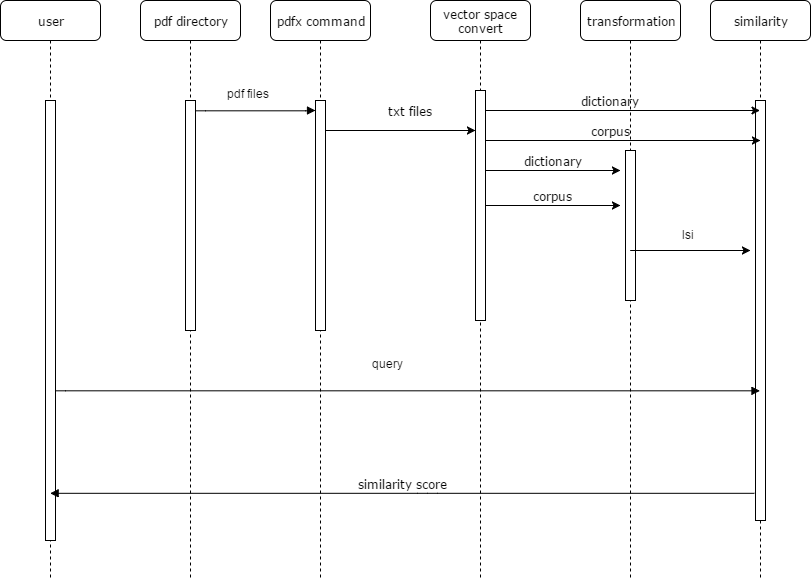
\includegraphics[width=0.9\textwidth]{Rainy_Sequence_diagram}
		\end{center}
		\caption{Sequence diagram of text similarity compare functionality.\label{Sequence diagram}}
	\end{figure*}
\newpage

	\section{Results and discussion}
We already have an interesting and hard working course. In the course, we build Django, PostgreSQL database, and develop search engine, after that we combine them together. Then, we can get the search result based on the search query. In order to have a user-friendly web page, we add some CSS programming files into it! We extend our database to 89 articles by manually downloading them from the Internet. Finally, we can display the similarity percentage and build a good-looking result page.

In brief, we have a functional web page implemented with search bar that you can copy a bunch of texts and return the percentage of similarity between the texts and the articles in the database.

	\section{Conclusions and future work}
    The results of this year are described below. We built a functional web server which contains full-text search function, similarity comparison, and the article hyperlink which can connect to the source website.
		
	%%%%%%%%%%%%%%%%%%%%%%%%%%%%%%%%%%%%%%%%%%%%%%%%%%%%%%%%%%%%%%%%%%%
	% References
	% Using Mendeley Desktop with library.bib
	%%%%%%%%%%%%%%%%%%%%%%%%%%%%%%%%%%%%%%%%%%%%%%%%%%%%%%%%%%%%%%%%%%%		
	\bibliographystyle{agsm_nurl}
	%\bibliography{library}	
	\clearpage 
\end{document}  
